Similar ao Seção \ref{sec:metastream}, os resultados são divididos em fases offline e online. Na avaliação offline, nós analisamos o meta-classificador a respeito do quão bem ele consegue discriminar as classes no nível meta. Na avaliação online, nós medimos os ganhos a respeito da performance preditiva no nível base quando aplicado a recomendação de algoritmos pelo meta-classificador.

\section{Analise Offline}

A Tabela \ref{tab:algo_dist} lista a distribuição de algoritmos (RF e SVM\footnote{Uma aproximação do SVM como descrito na seção metodologia.}) que apresentam a melhor performance para cada lote do fluxo de dados (\textit{Electricity}, \textit{CoverType}, \textit{PowerSupply}, \textit{HyperPlane}, \textit{Agrawal} e \textit{RandomRBF}). Na perspectiva de MtA, essa tabela apresenta a distribuição de classes dos meta-exemplos para os meta-dados offline.

\begin{table}[ht]
\caption{Distribuição de algoritmos nos meta-dados por problema de fluxo de dados.}
\label{tab:algo_dist}
\centering
\begin{tabular}{c|c|c} \hline
    Conjunto de Dados & SVM   & RF    \\ \hline
    Electricity       & 0.752 & 0.248 \\
    CoverType         & 0.718 & 0.282 \\
    PowerSupply       & 0.535 & 0.465 \\ \hline
    HyperPlane        & 0.792 & 0.207 \\
    Agrawal           & 0.785 & 0.215 \\
    RandomRBF         & 0.535 & 0.465 \\
\end{tabular}
\end{table}

Em termos gerais o algoritmo SVM apresentou melhor performance em relação ao RF para todos
os conjuntos de fluxos de dados. Para os conjuntos \textit{PowerSupply} e \textit{RandomRBF} a
performance foi quase balanceada entre eles. Já nos outros conjuntos a distribuição está bem
desbalanceada para o SVM, logo, treinamos o meta-classificador para que lidasse com esse
desbalanceamento,  ajustando a função custo em razão da proporção das classes. 

Nós então estimamos a performance preditiva do meta-classificador usando um validação cruzada para series temporais, como descrito em \cite{hyndman2018forecasting}, para os dados iniciais. O modelo é inicialmente induzido na primeira janela de $\omega_m=300$ exemplos de treino e prevê as classes dos próximos $\eta_m=10$ exemplos de teste, então ambas as janelas deslizam 1 exemplo para a próxima avaliação. A Tabela \ref{tab:offmetrics} apresenta a média e o desvio padrão para essas métricas. Ganhos da meta-recomendação advém da recomendação não trivial dos algoritmos. Dado que o método Padrão representa um Kappa igual a zero, $Kappa=0$, $Kappa > 0$ representa um ganho preditivo.


\begin{table}[ht]
\caption{Performance preditiva do meta-classificador na fase offline.}
\label{tab:offmetrics}
\centering
\begin{tabular}{c|c|c|c}\hline
    Fluxo   & Kappa           & M. Geométrica   & Acurácia        \\ \hline
Electricity & 0.095$\pm$0.176 & 0.366$\pm$0.207 & 0.610$\pm$0.152 \\
CoverType   & 0.018$\pm$0.215 & 0.329$\pm$0.232 & 0.517$\pm$0.147 \\
PowerSupply & 0.251$\pm$0.282 & 0.520$\pm$0.252 & 0.611$\pm$0.188 \\ \hline
HyperPlane  & 0.118$\pm$0.326 & 0.120$\pm$0.325 & 0.841$\pm$0.080 \\
Agrawal     & 0.007$\pm$0.138 & 0.046$\pm$0.164 & 0.780$\pm$0.078 \\
RandomRBF   & 0.120$\pm$0.239 & 0.416$\pm$0.262 & 0.571$\pm$0.115 \\
\end{tabular}
\end{table}

A Tabela \ref{tab:offmetrics} apresenta a performance preditiva da fase offline avaliadas por três medidas distintas na configuração de janela deslizante. A acurácia é estimada sobre $\eta_m=10$, que é comparável a distribuição dos meta-dados da Tabela \ref{tab:algo_dist}. Para as medidas Kappa e Média Geométrica, nós removemos os exemplos em $\eta_m$ onde não tiveram diferença significativa entre as performances dos algoritmos no nível base, isto é, nós computamos essas medidas para os exemplos base onde $|\text{Acc}(\text{RF})-\text{Acc}(\text{SVM})| > 0.1$. Essa abordagem foi aplicada com o objetivo de produzir uma mensuração mais apropriada do meta-classificador, pois onde não há uma diferença clara entre a performance dos modelos, qualquer um deles pode ser escolhido sem perdas.

Para todos os conjuntos, a medida Kappa é pelo menos levemente positiva, mostrando que o recomendador consegue selecionar o algoritmo correto quando há uma diferença significativa na performance preditiva entre eles, superando o método padrão. Acurácia é próxima da distribuição da classe majoritária, mas posteriormente iremos argumentar que grande parte dos exemplos não há diferença clara e alguns exemplos apresentam um ganho melhor de predição que outros, o que no nível base reflete em uma diferença significativa.

Para avaliar o quanto os meta-atributos contribuem ao sistema de recomendação, a Figura \ref{fig:fi} mostra os $5$ melhores meta-atributos, para cada conjunto, selecionado pelo algoritmo LightGBM. Nessa figura, o eixo $x$ representa a importância dos atributos dos meta-modelos dados pelo LightGBM, e o eixo $y$ mostra esses meta-atributos. A grande maioria dos meta-atributos selecionados por nós para dividir os dados foram do grupo de landmarking, seguido por baseado em modelo e estatístico. Esses grupos tem o maior grau informativo e discriminativo de acordo com a literatura \cite{Rivolli2018}.

\begin{figure}[ht]
    \centering
    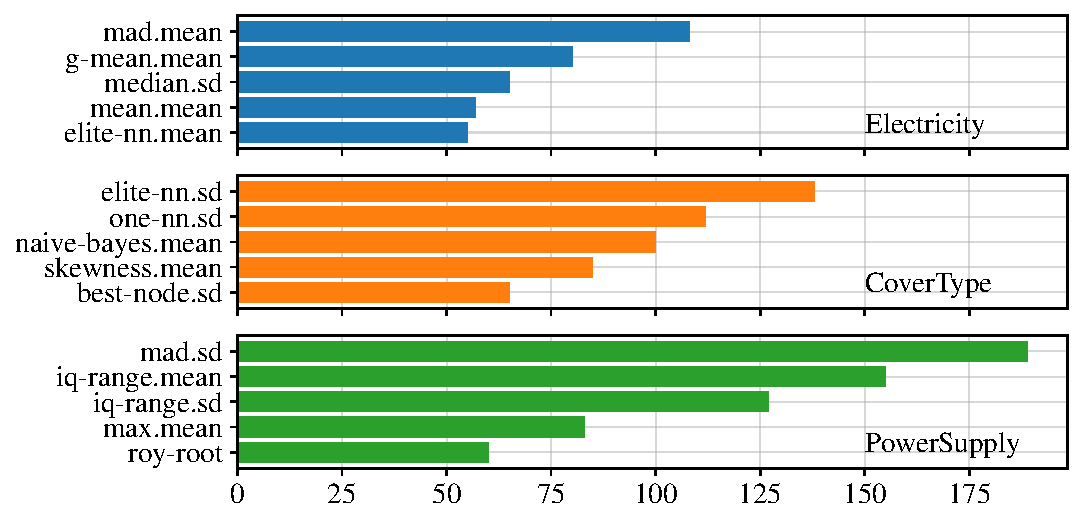
\includegraphics[width=0.8\linewidth]{general_fi}
    \caption{Importância dos atributos para o meta-algoritmo nos dados offline.}
    \label{fig:fi}
\end{figure}


\section{Analise Online}

Na fase online, nós avaliamos o meta-classificador (LightGBM) usando uma estratégia incremental e não incremental. Na avaliação passada, nós treinamos o meta-classificador usando o procedimento descrito na Seção \ref{subsec:online}. Quando novos meta-atributos estão disponíveis, o meta-classificador e retreinado do zero, e isto pode levar a um modelo completamente independente do modelo passado. Na estratégia online, o LightGBM atualiza o modelo anterior, adaptando as árvores de decisão para se ajustar aos meta-exemplos da janela mais recente, atualizando assim os pesos de cada nó, mas sem substitui-los. A Tabela \ref{tab:onmetrics} apresenta esses resultados.


\begin{table}[ht]
\caption{Performance preditiva do meta-classificador na fase online.}
\label{tab:onmetrics}
\centering
\begin{tabular}{r|l|c|c|c} \hline
Dataset     &  Estratégia    & Kappa & M. Geométrica & Acurácia \\ \hline
\multirow{2}{*}{Electricity} &  Non-Incremental      & 0.027 & 0.462  & 0.558    \\
            &  Incremental & 0.039 & 0.422  & 0.457    \\ \hline
\multirow{2}{*}{CoverType}   &  Non-Incremental       & 0.114 & 0.461  & 0.694    \\
            &  Incremental & -0.009 & 0.405  & 0.631    \\ \hline
\multirow{2}{*}{PowerSupply} &  Non-Incremental      & 0.092 & 0.502  & 0.607    \\
            &  Incremental & 0.074 & 0.541  & 0.539 \\ \hline
\multirow{2}{*}{HyperPlane}   &  Non-Incremental       & 0.014 & 0.265  & 0.747    \\
            &  Incremental & 0.020 & 0.283  & 0.745    \\ \hline
\multirow{2}{*}{Agrawal}   &  Non-Incremental       & 0.010 & 0.198  & 0.794    \\
            &  Incremental & -0.041 & 0.327  & 0.700    \\ \hline
\multirow{2}{*}{RandomRBF}   &  Non-Incremental       & -0.031 & 0.484  & 0.484    \\
            &  Incremental & 0.004 & 0.486  & 0.501
\end{tabular}
\end{table}

Embora a Tabela \ref{tab:onmetrics} apresente valores para Kappa relativamente baixos, nós notamos que esse valor é positivo para quase todas as combinações de conjunto-estratégia. Esses resultados indicam que o meta-classificador consegue selecionar o algoritmo mais apropriado comparado com a classe majoritária. Esse resultado é mais evidente para o conjunto \textit{PowerSupply}, que apresenta a melhor média geométrica e Kappa. Essa consistência refletirá posteriormente nos ganhos acumulados para esse conjunto. A estratégia incremental apresenta melhores performances em relação a não incremental para os conjuntos \textit{Electricity}, \textit{HyperPlane} e \textit{RandomRBF}, para os outros conjuntos o incremental performou pior para essas métricas.

Figuras \ref{fig:cumsum_elec2}-\ref{fig:cumsum_powersupply} mostram o ganho cumulativo, que é a diferença entre a acurácia do algoritmo recomendado e a acurácia do método Padrão. A região preenchida é a soma aculumada dessas diferenás de escore ao longo do tempo enquanto as cores laranja e azul representam as estratégias incrementais e não incrementais, respectivamente. Cada ponto preto representa o ganho de escore no tempo $t$.

\begin{figure}[!t]
    \centering
    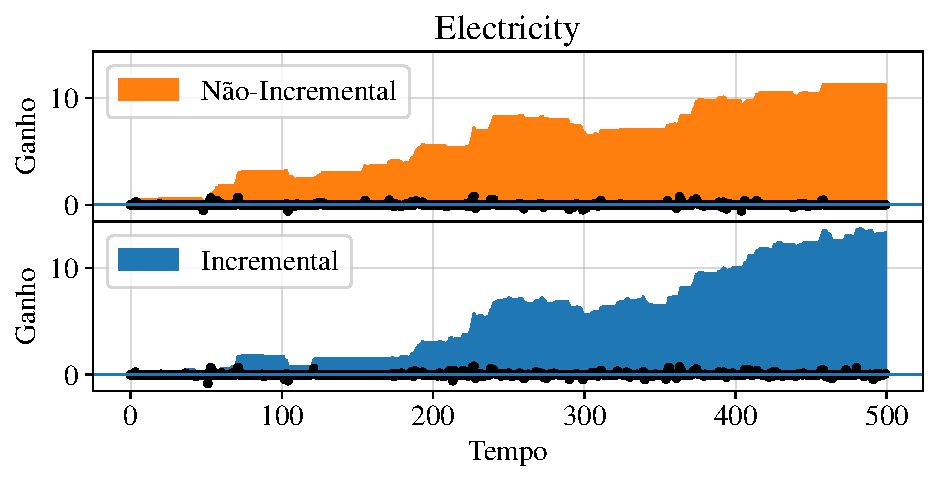
\includegraphics[width=0.8\linewidth]{elec2_cumsum}
    \caption{Ganho cumulativo de escore ao longo do tempo para o conjunto Electricity.}
    \label{fig:cumsum_elec2}
\end{figure}

\begin{figure}[!t]
    \centering
    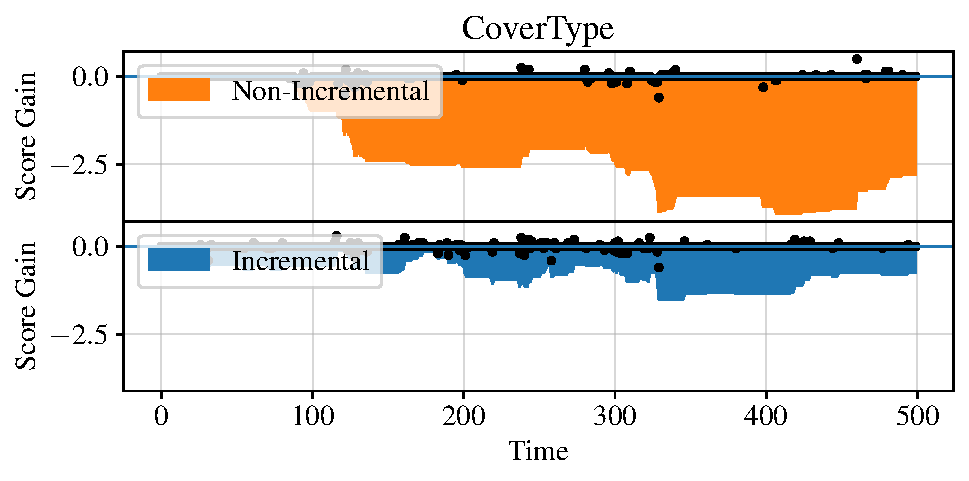
\includegraphics[width=0.8\linewidth]{covtype_cumsum}
    \caption{Ganho cumulativo de escore ao longo do tempo para o conjunto CoverType.}
    \label{fig:cumsum_covtype}
\end{figure}

\begin{figure}[!t]
    \centering
    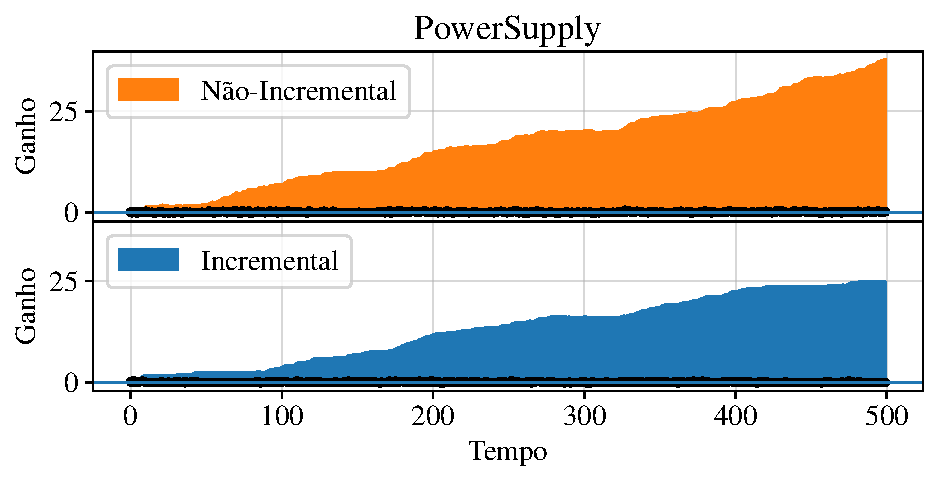
\includegraphics[width=0.8\linewidth]{powersupply_cumsum}
    \caption{Ganho cumulativo de escore ao longo do tempo para o conjunto PowerSupply.}
    \label{fig:cumsum_powersupply}
\end{figure}


In these figures, we observe a positive gain for the \textit{Electricity} and \textit{PowerSupply} datasets considering the recommendations of both strategies. However, the incremental strategy presents better performance for \textit{Electricity} as opposed to \textit{PowerSupply}, where the non-incremental is slightly better. In the \textit{CoverType} dataset we notice an interesting aspect. The non-incremental strategy presents a greater gain compared to the incremental one for lower points in time, but around $t=450$, it starts to make incorrect recommendations. On the contrary, the incremental strategy is more constant, keeping gains slightly over time after $t-300$. This is partly determined by the difficulty of the dataset, mainly after $t-400$, since the label that should be learned to infer the next window is not present in the training data.  This is particularly difficult for the non-incremental strategy since the incremental one keeps the past learned target information.


\begin{figure}[!t]
    \centering
    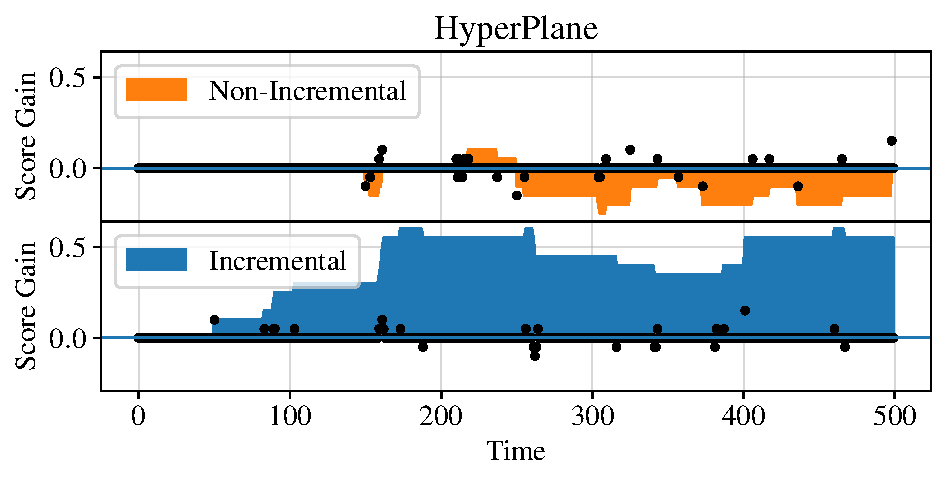
\includegraphics[width=0.8\linewidth]{hyper_cumsum}
    \caption{Ganho cumulativo de escore ao longo do tempo para o conjunto HyperPlane.}
    \label{fig:cumsum_hyper}
\end{figure}

\begin{figure}[!t]
    \centering
    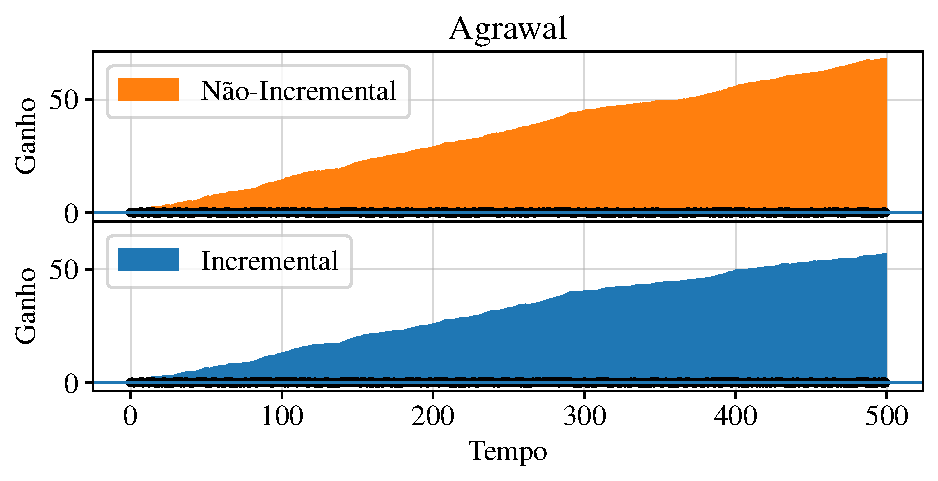
\includegraphics[width=0.8\linewidth]{agrawal_cumsum}
    \caption{Ganho cumulativo de escore ao longo do tempo para o conjunto Agrawal.}
    \label{fig:cumsum_agrawal}
\end{figure}

\begin{figure}[!t]
    \centering
    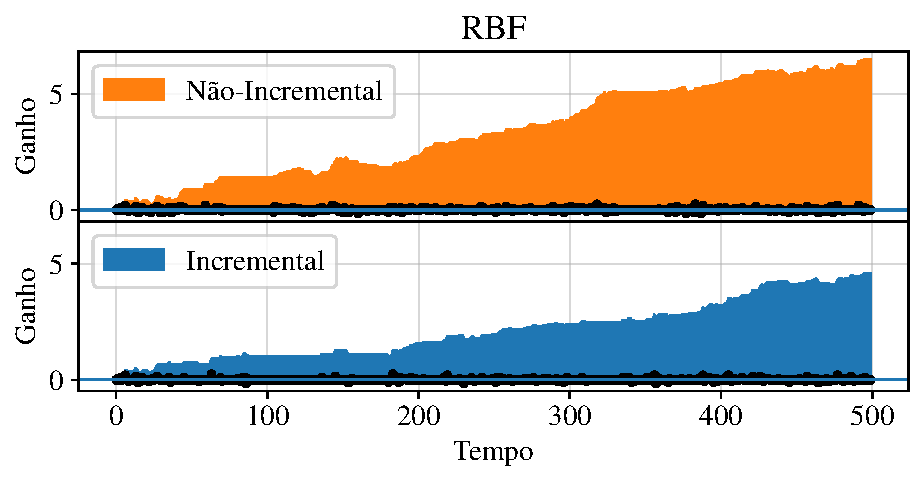
\includegraphics[width=0.8\linewidth]{rbf_cumsum}
    \caption{Ganho cumulativo de escore ao longo do tempo para o conjunto RandomRBF.}
    \label{fig:cumsum_rbf}
\end{figure}

In Figures \ref{fig:scorecross_elec2}, \ref{fig:scorecross_covtype} and \ref{fig:scorecross_powersupply} the scores from Default are plotted against the scores from the recommended algorithms in a 2-dimensional histogram heatmap.
Thus, each square in the heatmap represents the accuracy of the algorithm recommended by the Default method ($x$ axis) and the meta-classifier ($y$ axis) for the same window. The colour intensity as shown in the colour bar represents the number of points in that position. The points in the diagonal, where the recommended algorithm and the default algorithm had the same accuracy score, were removed and coloured as white to emphasize gains or losses of the framework.
If the recommended classifier is always worse than the Default, i.e., recommending the minority class when it is not better than the majority, then all points will be below the white diagonal. Similarly, these points will be above if it is effectively selecting the algorithm from minority class when it is better than the majority.

\begin{figure}[!t]
    \centering
    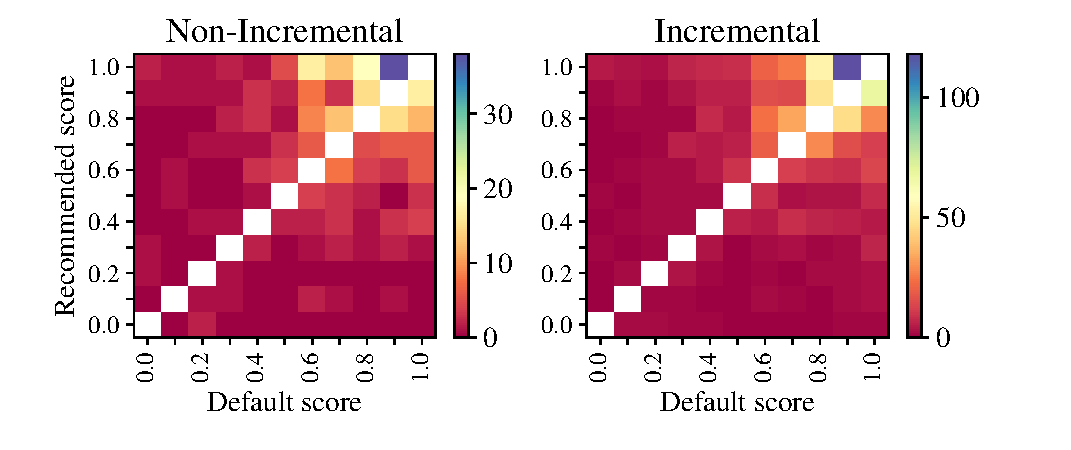
\includegraphics[width=0.8\linewidth]{elec2_score}
    \caption{Comparison between recommended and Default for Electricity.}
    \label{fig:scorecross_elec2}
\end{figure}

In Figure \ref{fig:scorecross_elec2}, it is visible in the upper right region of the heatmap that the incremental algorithm is recommending the minority class more often than the incremental one, also the blue square above the white diagonal has many more points (80 compared to 30 in the non-incremental), this reflects in gains as shown in Figure \ref{fig:cumsum_elec2}.

\begin{figure}[!t]
    \centering
    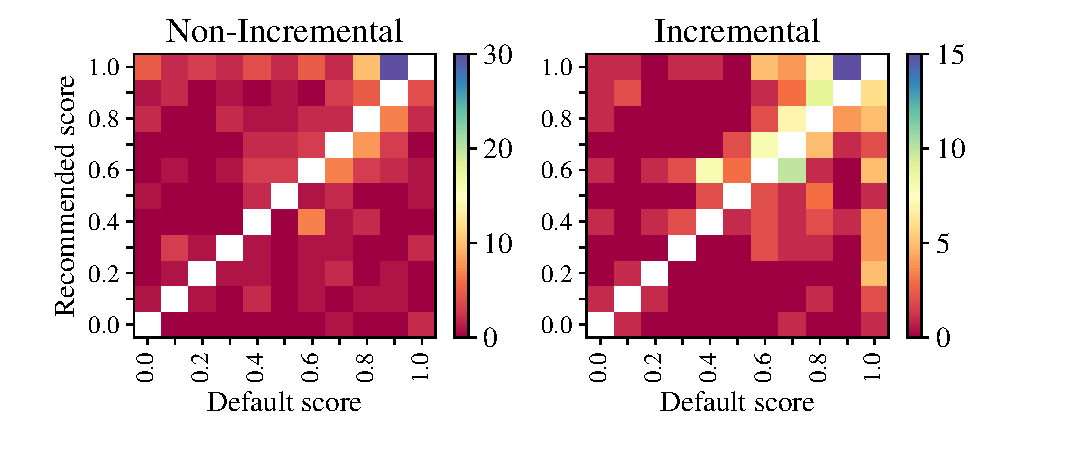
\includegraphics[width=0.8\linewidth]{covtype_score}
    \caption{Comparison between recommended and Default for CoverType.}
    \label{fig:scorecross_covtype}
\end{figure}

For the \textit{Covertype} (Figure \ref{fig:scorecross_covtype}), we observe a different behaviour, there is a blue square above the diagonal for the non-incremental plot and a blue square below the diagonal in the incremental one. This points out that the incremental recommendation is performing worse than the default, as could be seen in Figure \ref{fig:cumsum_covtype}. The non-incremental also presents some light coloured squares below the diagonal, which resulted in reduced overall performance for later points in time.

\begin{figure}[!t]
    \centering
    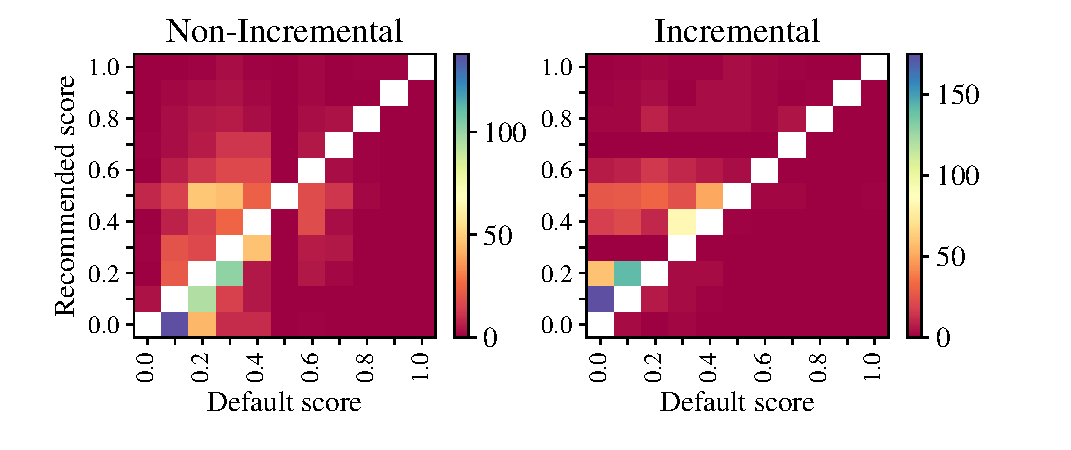
\includegraphics[width=0.8\linewidth]{powersupply_score}
    \caption{Comparison between recommended and Default for PowerSupply.}
    \label{fig:scorecross_powersupply}
\end{figure}

The \textit{PowerSupply} dataset, which has 24 classes, is the hardest one to classify, since all points are below 0.8 accuracy as shown in Figure \ref{fig:scorecross_powersupply}. However, in the meta-level, was easier to discriminate algorithms as the meta-data is balanced, reflecting in a less symmetrical distribution for the diagonal (the upper region is more populated), it is also confirmed in Figure \ref{fig:cumsum_powersupply}, with the highest cumulative score gain amongst the datasets.

\begin{figure}[!t]
    \centering
    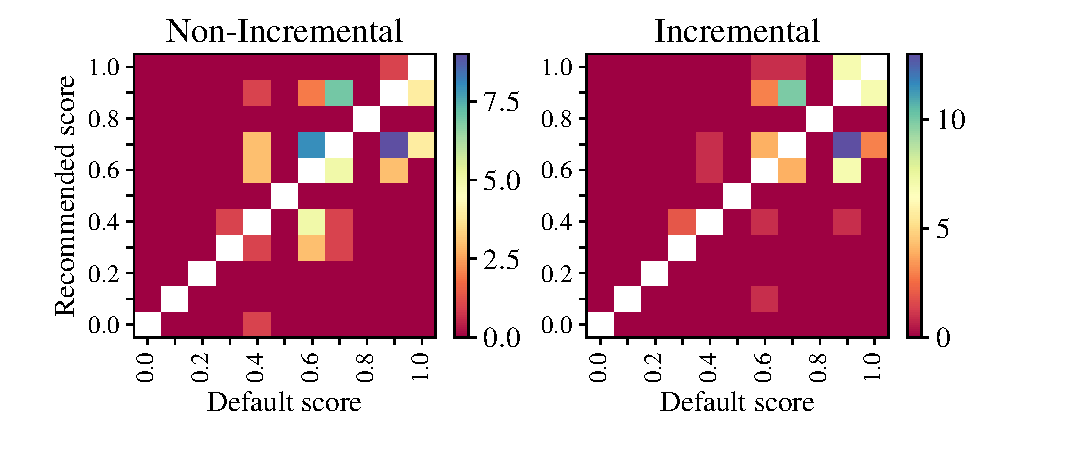
\includegraphics[width=0.8\linewidth]{hyper_score}
    \caption{Comparison between recommended and Default for HyperPlane.}
    \label{fig:scorecross_hyper}
\end{figure}

\begin{figure}[!t]
    \centering
    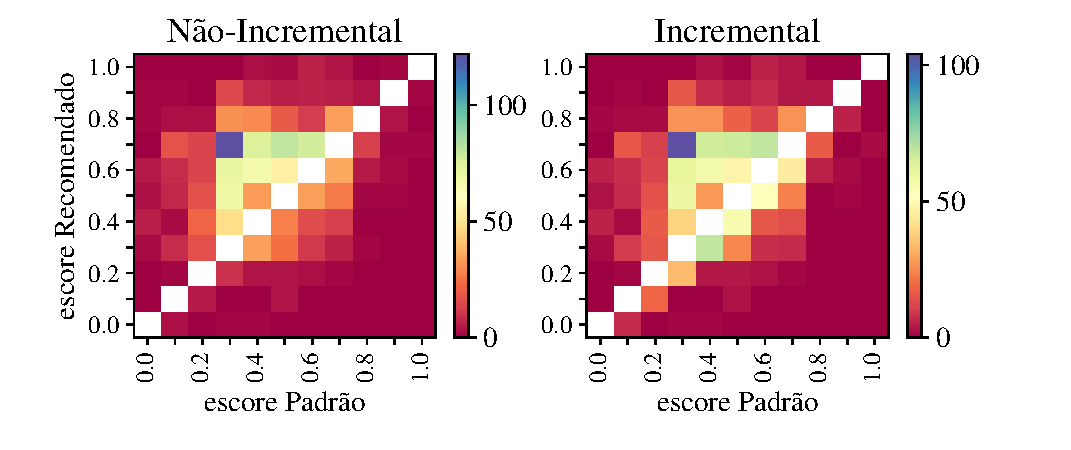
\includegraphics[width=0.8\linewidth]{agrawal_score}
    \caption{Comparison between recommended and Default for Agrawal.}
    \label{fig:scorecross_agrawal}
\end{figure}

\begin{figure}[!t]
    \centering
    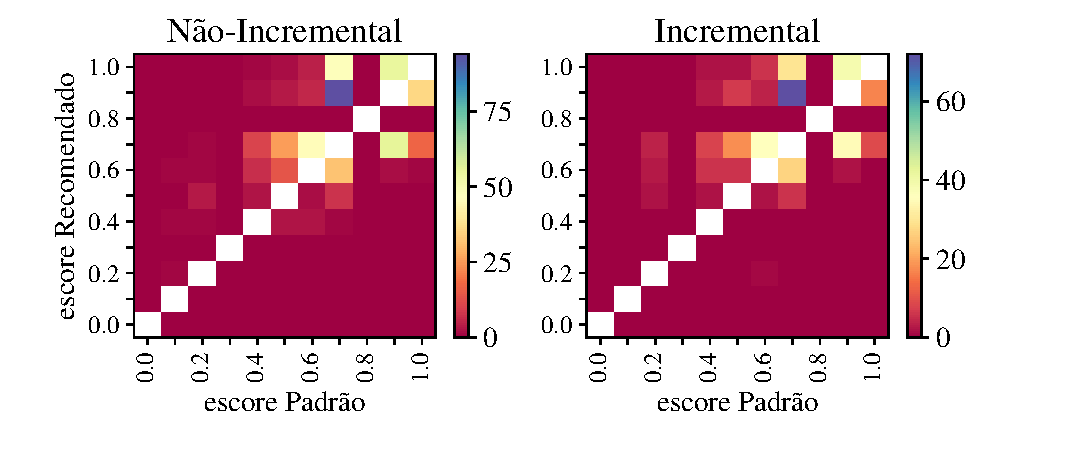
\includegraphics[width=0.8\linewidth]{rbf_score}
    \caption{Comparison between recommended and Default for RandomRBF.}
    \label{fig:scorecross_rbf}
\end{figure}


\begin{figure}[!t]
    \centering
    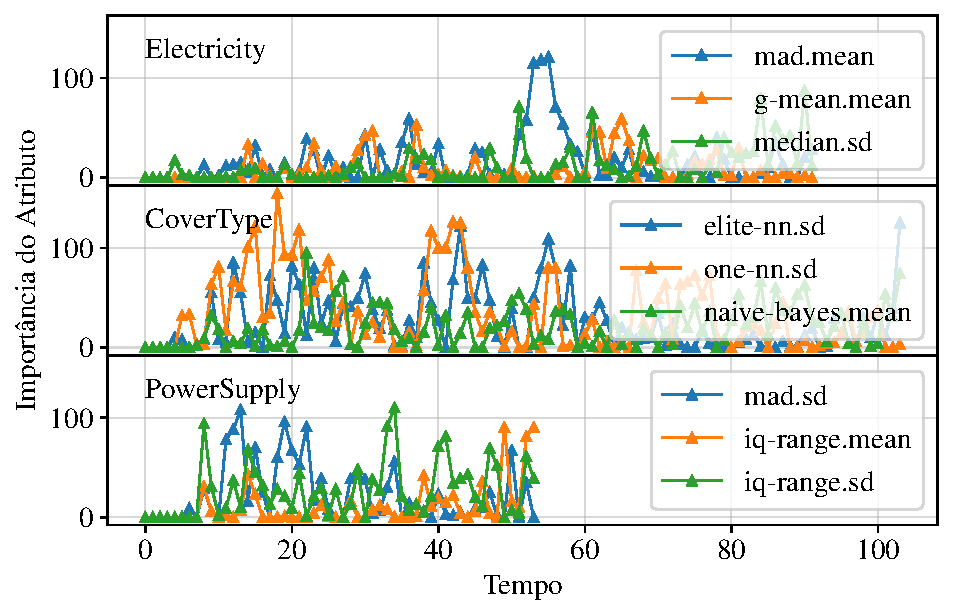
\includegraphics[width=0.8\linewidth]{general_timefi}
    \caption{Variation in feature importance over time for three meta-features.}
    \label{fig:fi_time}
\end{figure}

The feature importance for the non-incremental strategy is given by Figure \ref{fig:fi}, as it keeps the same nodes obtained by training in the offline meta-data. The main difference between incremental and batch learning for this problem is that the feature importance is fixed in incremental learning. However, as shown in Figure \ref{fig:fi_time}, the importance varies for each trained window. It is believed that fixing feature importance acts as a regularization. Still, alternatively, concept drift could also occur in the meta-level, being this possibly beneficial to have a flexible tree choice.